\documentclass{article}

\usepackage{courier}
\usepackage{listings}
\usepackage{graphicx}
\usepackage{xcolor}
\usepackage{colortbl}
\usepackage{multirow}
\usepackage{longtable}
\usepackage{fontspec} 
\usepackage{polyglossia}
\usepackage{lastpage}
\usepackage{ifthen}

\usepackage[
    paper=a4paper,
    tmargin=2.5cm,
    bmargin=2.5cm,
    lmargin=2.5cm,
    rmargin=2.5cm]{geometry}
\usepackage{fancyhdr}
\pagestyle{fancy}
\usepackage{bookmark}
\usepackage{parskip}

\usepackage{xeCJK}
\setCJKmainfont{SimSun} 

\def\versionplantuml{1.2025.0}

\hypersetup{
	colorlinks=true,
	linkcolor=black,
	pdfsubject={Drawing UML with PlantUML},
	pdftitle={PlantUML Language Reference Guide},
	pdfkeywords={UML}
}

\rfoot{\thepage\ / \pageref{LastPage}}
\lfoot{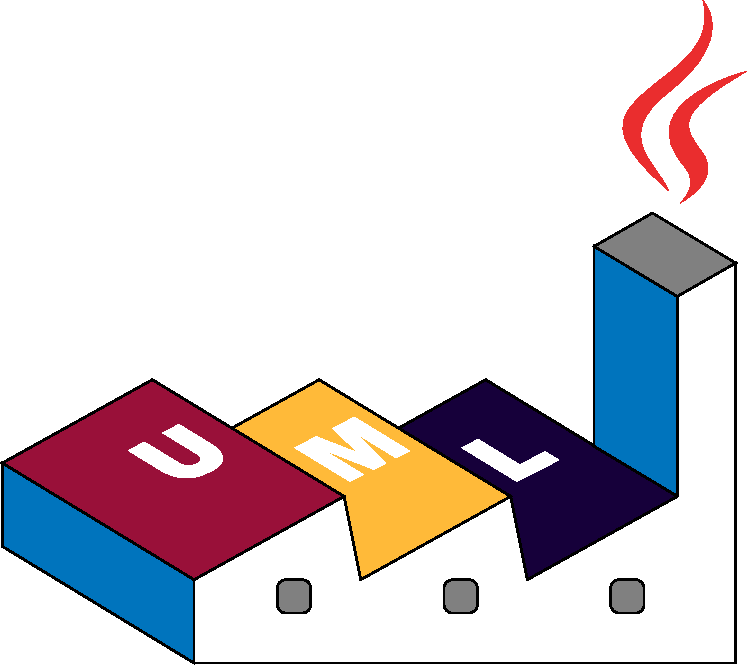
\includegraphics[width=7mm]{Logo_PlantUML.pdf}\hspace{3mm}\textit{PlantUML Language Reference Guide (\versionplantuml)}}
\cfoot{}

\lstset{basicstyle=\footnotesize\ttfamily}

\author{PlantUML}
\title{Drawing UML with PlantUML}

\begin{document}

\begin{titlepage}
	\begin{center}
		\Huge{Drawing UML with PlantUML}
		\vskip 5mm
		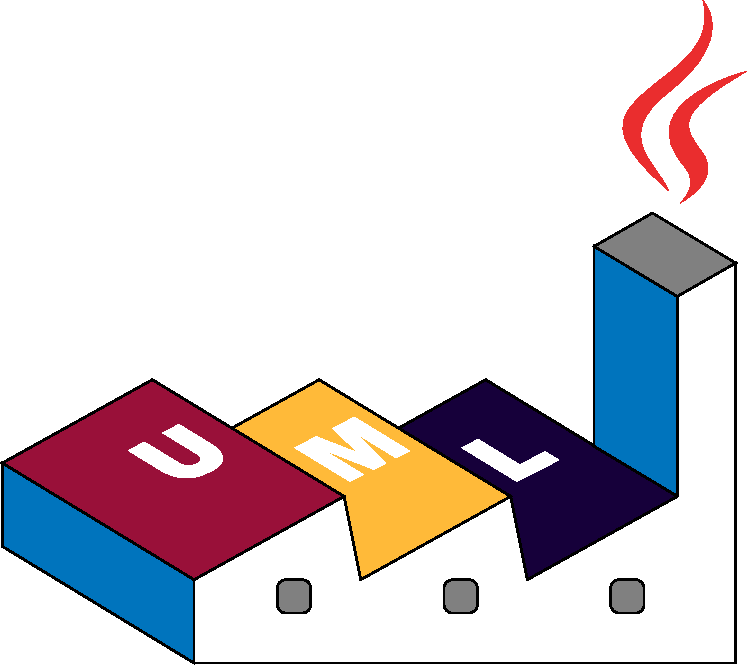
\includegraphics[width=30mm]{Logo_PlantUML.pdf}
		\vskip 5mm
		\Large{PlantUML Language Reference Guide}
		\vskip 1mm
		\large{(Version \versionplantuml)}
	\end{center}

	\vskip 2cm
\textbf{PlantUML} is a component that allows to quickly write :


\begin{itemize}
\item Sequence diagram
\item Usecase diagram
\item Class diagram
\item Object diagram
\item Activity diagram
\item Component diagram
\item Deployment diagram
\item State diagram
\item Timing diagram
\end{itemize}


The following non-UML diagrams are also supported:

\begin{itemize}
\item JSON Data
\item YAML Data
\item Network diagram (nwdiag)
\item Wireframe graphical interface
\item Archimate diagram
\item Specification and Description Language (SDL)
\item Ditaa diagram
\item Gantt diagram
\item MindMap diagram 
\item Work Breakdown Structure diagram 
\item Mathematic with AsciiMath or JLaTeXMath notation
\item Entity Relationship diagram
\end{itemize}

Diagrams are defined using a simple and intuitive language.	
\end{titlepage}


%%
% Sequence Diagram
%
\section{Sequence Diagram}


Creating sequence diagrams with PlantUML is remarkably straightforward. This ease of use is largely attributed to the user-friendly nature of its syntax, designed to be both intuitive and easy to remember.


\begin{itemize}
\item \textbf{Intuitive Syntax:} 
\end{itemize}
  First and foremost, users appreciate the straightforward and intuitive syntax that PlantUML employs. This well-thought-out design means that even those new to diagram creation find it easy to grasp the basics quickly and without hassle.


\begin{itemize}
\item \textbf{Text-to-Graphic Correlation:} 
\end{itemize}
  Another distinguishing feature is the close resemblance between the textual representation and the graphical output. This harmonious correlation ensures that the textual drafts translate quite accurately into graphical diagrams, providing a cohesive and predictable design experience without unpleasant surprises in the final output.


\begin{itemize}
\item \textbf{Efficient Crafting Process:} 
\end{itemize}
  The strong correlation between the text and the graphical result not only simplifies the crafting process but also significantly speeds it up. Users benefit from a more streamlined process with fewer requirements for time-consuming revisions and adjustments.


\begin{itemize}
\item \textbf{Visualization While Drafting:} 
\end{itemize}
  The ability to envisage the final graphical outcome while drafting the text is a feature that many find invaluable. It naturally fosters a smooth transition from initial draft to final presentation, enhancing productivity and reducing the likelihood of errors.


\begin{itemize}
\item \textbf{Easy Edits and Revisions:} 
\end{itemize}
  Importantly, editing existing diagrams is a hassle-free process. Since the diagrams are generated from text, users find that making adjustments is considerably easier and more precise than altering an image using graphical tools. It boils down to simply modifying the text, a process far more straightforward and less prone to errors than making changes through a graphical interface with a mouse.


PlantUML facilitates a straightforward and user-friendly approach to creating and editing sequence diagrams, meeting the needs of both novices and seasoned designers alike. It skillfully leverages the simplicity of textual inputs to craft visually descriptive and accurate diagrams, thereby establishing itself as a must-have tool in the diagram creation toolkit.


You can learn more about some of the common commands in PlantUML to enhance your diagram creation experience.
%
% Basic Examples
%
\subsection{Basic Examples}


In PlantUML sequence diagrams, the \texttt{->} sequence denotes a message sent between two participants, which are automatically recognized and do not need to be declared beforehand.


Utilize dotted arrows by employing the \texttt{-->} sequence, offering a distinct visualization in your diagrams.


To improve readability without affecting the visual representation, use reverse arrows like \texttt{<-} or \texttt{<--}. However, be aware that this is specifically for sequence diagrams and the rules differ for other diagram types.




\begin{verbatim}
@startuml
Alice -> Bob: Authentication Request
Bob --> Alice: Authentication Response

Alice -> Bob: Another authentication Request
Alice <-- Bob: Another authentication Response
@enduml
\end{verbatim}
% true imgw/img-63d99af67915f6505d4c3222c3e0b010.png
\begin{center}
% image width = 267
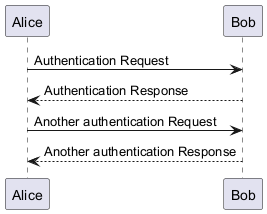
\includegraphics[scale=0.60]{imgw/img-63d99af67915f6505d4c3222c3e0b010.png}
\end{center}
%
% Declaring participant
%
\subsection{Declaring participant}


If the keyword \texttt{participant} is used to declare a participant, more control on that participant is possible.


The order of declaration will be the (default) \textbf{order of display}.


Using these other keywords to declare participants will \textbf{change the shape} of the participant representation:
\begin{itemize}
\item \texttt{actor}
\item \texttt{boundary}
\item \texttt{control}
\item \texttt{entity}
\item \texttt{database}
\item \texttt{collections}
\item \texttt{queue}
\end{itemize}


\begin{verbatim}
@startuml
participant Participant as Foo
actor       Actor       as Foo1
boundary    Boundary    as Foo2
control     Control     as Foo3
entity      Entity      as Foo4
database    Database    as Foo5
collections Collections as Foo6
queue       Queue       as Foo7
Foo -> Foo1 : To actor 
Foo -> Foo2 : To boundary
Foo -> Foo3 : To control
Foo -> Foo4 : To entity
Foo -> Foo5 : To database
Foo -> Foo6 : To collections
Foo -> Foo7: To queue
@enduml
\end{verbatim}
% true imgw/img-aab53771966850933e74522259169424.png
\begin{center}
% image width = 574
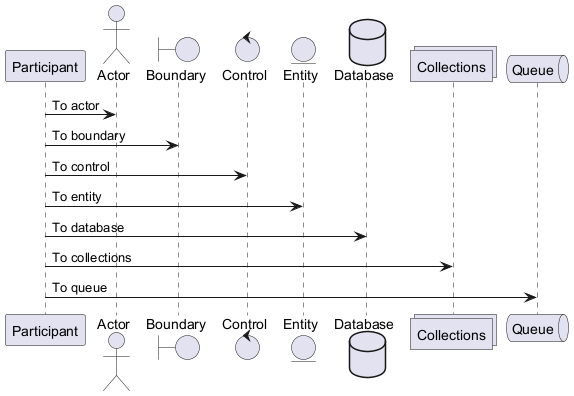
\includegraphics[scale=0.60]{imgw/img-aab53771966850933e74522259169424.png}
\end{center}


Rename a participant using the \texttt{as} keyword.


You can also change the background color of
actor or participant.


\begin{verbatim}
@startuml
actor Bob #red
' The only difference between actor
'and participant is the drawing
participant Alice
participant "I have a really\nlong name" as L #99FF99
/' You can also declare:
   participant L as "I have a really\nlong name"  #99FF99
  '/

Alice->Bob: Authentication Request
Bob->Alice: Authentication Response
Bob->L: Log transaction
@enduml
\end{verbatim}
% true imgw/img-c5cddd003652cd1b3109cdc71b9987d8.png
\begin{center}
% image width = 327
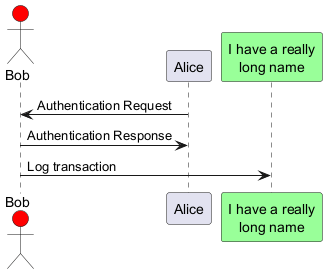
\includegraphics[scale=0.60]{imgw/img-c5cddd003652cd1b3109cdc71b9987d8.png}
\end{center}


You can use the \texttt{order} keyword to customize the display order of participants.


\begin{verbatim}
@startuml
participant Last order 30
participant Middle order 20
participant First order 10
@enduml
\end{verbatim}
% true imgw/img-65dfd7ae9330e7e48e090871dc8b601f.png
\begin{center}
% image width = 166
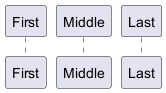
\includegraphics[scale=0.60]{imgw/img-65dfd7ae9330e7e48e090871dc8b601f.png}
\end{center}
%
% Declaring participant on multiline
%
\subsection{Declaring participant on multiline}


You can declare participant on multi-line.


\begin{verbatim}
@startuml
participant Participant [
    =Title
    ----
    ""SubTitle""
]

participant Bob

Participant -> Bob
@enduml
\end{verbatim}
% true imgw/img-2aeb582e872a4b823c6ed833d727d9a1.png
\begin{center}
% image width = 140
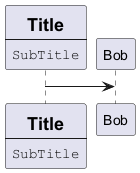
\includegraphics[scale=0.60]{imgw/img-2aeb582e872a4b823c6ed833d727d9a1.png}
\end{center}


\textit{[Ref. QA-15232]}
%
% Use non-letters in participants
%
\subsection{Use non-letters in participants}




You can use quotes to define participants.
And you can use the \texttt{as} keyword to give an alias to those participants.
\begin{verbatim}
@startuml
Alice -> "Bob()" : Hello
"Bob()" -> "This is very\nlong" as Long
' You can also declare:
' "Bob()" -> Long as "This is very\nlong"
Long --> "Bob()" : ok
@enduml
\end{verbatim}
% true imgw/img-c49b682a2712ca0450d139146bf5eb11.png
\begin{center}
% image width = 207
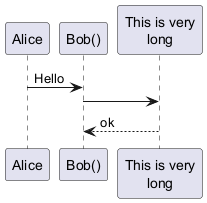
\includegraphics[scale=0.60]{imgw/img-c49b682a2712ca0450d139146bf5eb11.png}
\end{center}


%
% Message to Self
%
\subsection{Message to Self}


A participant can send a message to itself.


It is also possible to have multi-line using \texttt{\textbackslash n}.


\begin{verbatim}
@startuml
Alice -> Alice: This is a signal to self.\nIt also demonstrates\nmultiline \ntext
@enduml
\end{verbatim}
% true imgw/img-83e0a2ff75504a63c1db6b286565bf38.png
\begin{center}
% image width = 168
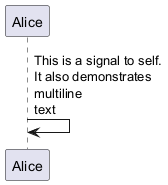
\includegraphics[scale=0.60]{imgw/img-83e0a2ff75504a63c1db6b286565bf38.png}
\end{center}


\begin{verbatim}
@startuml
Alice <- Alice: This is a signal to self.\nIt also demonstrates\nmultiline \ntext
@enduml
\end{verbatim}
% true imgw/img-395f23eec190f589f05ca92c5ba19f8d.png
\begin{center}
% image width = 169
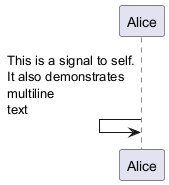
\includegraphics[scale=0.60]{imgw/img-395f23eec190f589f05ca92c5ba19f8d.png}
\end{center}
\textit{[Ref. QA-1361]}
%
% Text alignment
%
\subsection{Text alignment}


Text alignment on arrows can be set to \texttt{left}, \texttt{right} or \texttt{center} using \texttt{skinparam sequenceMessageAlign}. 


You can also use \texttt{direction} or \texttt{reverseDirection} to align text depending on arrow direction. Further details and examples of this are available on the skinparam page.


\begin{verbatim}
@startuml
skinparam sequenceMessageAlign right
Bob -> Alice : Request
Alice -> Bob : Response
@enduml
\end{verbatim}
% true imgw/img-2bcb9c2980c5243ee4aefe834849bbf5.png
\begin{center}
% image width = 134
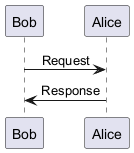
\includegraphics[scale=0.60]{imgw/img-2bcb9c2980c5243ee4aefe834849bbf5.png}
\end{center}


\subsubsection{Text of response message below the arrow}


You can put the text of the response message below the arrow, with the \texttt{skinparam responseMessageBelowArrow true} command.


\begin{verbatim}
@startuml
skinparam responseMessageBelowArrow true
Bob -> Alice : hello
Bob <- Alice : ok
@enduml
\end{verbatim}
% true imgw/img-47439438c617287f7b5c1619b3c72ae2.png
\begin{center}
% image width = 103
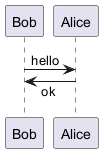
\includegraphics[scale=0.60]{imgw/img-47439438c617287f7b5c1619b3c72ae2.png}
\end{center}
%
% Change arrow style
%
\subsection{Change arrow style}


You can change arrow style by several ways:
\begin{itemize}
\item add a final \texttt{x} to denote a lost message
\item use \texttt{\textbackslash} or \texttt{/} instead of \texttt{<} or \texttt{>} to have only the bottom or top part of the arrow
\item repeat the arrow head (for example, \texttt{>>} or \texttt{//}) head to have a thin drawing
\item use \texttt{--} instead of \texttt{-} to have a dotted arrow
\item add a final "o" at arrow head
\item use bidirectional arrow \texttt{<->}
\end{itemize}


\begin{verbatim}
@startuml
Bob ->x Alice
Bob -> Alice
Bob ->> Alice
Bob -\ Alice
Bob \\- Alice
Bob //-- Alice

Bob ->o Alice
Bob o\\-- Alice

Bob <-> Alice
Bob <->o Alice
@enduml
\end{verbatim}
% true imgw/img-7a5cf483763182898a9e0e6a62a39a7f.png
\begin{center}
% image width = 103
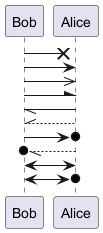
\includegraphics[scale=0.60]{imgw/img-7a5cf483763182898a9e0e6a62a39a7f.png}
\end{center}


%
% Change arrow color
%
\subsection{Change arrow color}


You can change the color of individual arrows using the following notation:
\begin{verbatim}
@startuml
Bob -[#red]> Alice : hello
Alice -[#0000FF]->Bob : ok
@enduml
\end{verbatim}
% true imgw/img-a0b5a4d9c1c477ceec2d11f1b490c0ba.png
\begin{center}
% image width = 103
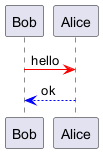
\includegraphics[scale=0.60]{imgw/img-a0b5a4d9c1c477ceec2d11f1b490c0ba.png}
\end{center}


%
% Message sequence numbering
%
\subsection{Message sequence numbering}




The keyword \texttt{autonumber} is used to
automatically add an incrementing number to messages.


\begin{verbatim}
@startuml
autonumber
Bob -> Alice : Authentication Request
Bob <- Alice : Authentication Response
@enduml
\end{verbatim}
% true imgw/img-798952cd30f576175cca17a4075180d9.png
\begin{center}
% image width = 231
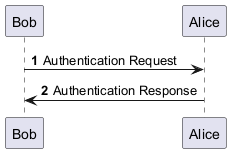
\includegraphics[scale=0.60]{imgw/img-798952cd30f576175cca17a4075180d9.png}
\end{center}


You can specify a startnumber with \texttt{autonumber <start>} , and
also an increment with \texttt{autonumber <start> <increment>}.




\begin{verbatim}
@startuml
autonumber
Bob -> Alice : Authentication Request
Bob <- Alice : Authentication Response

autonumber 15
Bob -> Alice : Another authentication Request
Bob <- Alice : Another authentication Response

autonumber 40 10
Bob -> Alice : Yet another authentication Request
Bob <- Alice : Yet another authentication Response

@enduml
\end{verbatim}
% true imgw/img-bb76bd00dba7cddb71dfe94cabccc9be.png
\begin{center}
% image width = 308
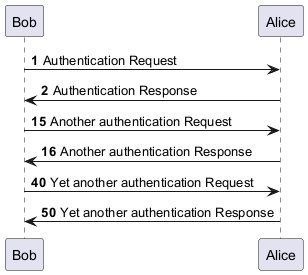
\includegraphics[scale=0.60]{imgw/img-bb76bd00dba7cddb71dfe94cabccc9be.png}
\end{center}




You can specify a format for your number by using between double-quote.


The formatting is done with the Java class \texttt{DecimalFormat}
(\texttt{0} means digit, \texttt{\#} means digit and zero if absent).


You can use some html tag in the format.
\begin{verbatim}
@startuml
autonumber "<b>[000]"
Bob -> Alice : Authentication Request
Bob <- Alice : Authentication Response

autonumber 15 "<b>(<u>##</u>)"
Bob -> Alice : Another authentication Request
Bob <- Alice : Another authentication Response

autonumber 40 10 "<font color=red><b>Message 0  "
Bob -> Alice : Yet another authentication Request
Bob <- Alice : Yet another authentication Response

@enduml
\end{verbatim}
% true imgw/img-7fc6f31227ef57c7a3e87600375a7ed6.png
\begin{center}
% image width = 373
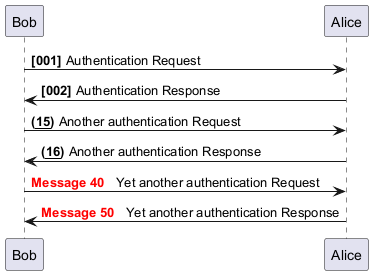
\includegraphics[scale=0.60]{imgw/img-7fc6f31227ef57c7a3e87600375a7ed6.png}
\end{center}


You can also use \texttt{autonumber stop} and
\texttt{autonumber resume <increment> <format>} to respectively pause and resume
automatic numbering.


\begin{verbatim}
@startuml
autonumber 10 10 "<b>[000]"
Bob -> Alice : Authentication Request
Bob <- Alice : Authentication Response

autonumber stop
Bob -> Alice : dummy

autonumber resume "<font color=red><b>Message 0  "
Bob -> Alice : Yet another authentication Request
Bob <- Alice : Yet another authentication Response

autonumber stop
Bob -> Alice : dummy

autonumber resume 1 "<font color=blue><b>Message 0  "
Bob -> Alice : Yet another authentication Request
Bob <- Alice : Yet another authentication Response
@enduml
\end{verbatim}
% true imgw/img-0d05e1597b1eff1b6e8a7f72af608928.png
\begin{center}
% image width = 373
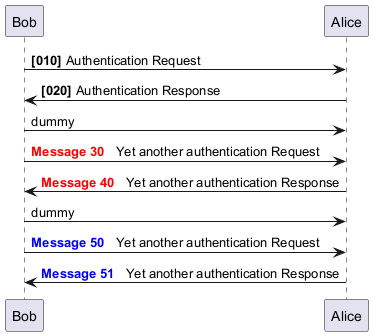
\includegraphics[scale=0.60]{imgw/img-0d05e1597b1eff1b6e8a7f72af608928.png}
\end{center}


Your startnumber can also be a 2 or 3 digit sequence using a field delimiter such as \texttt{.}, \texttt{;}, \texttt{,}, \texttt{:} or a mix of these. For example: \texttt{1.1.1} or \texttt{1.1:1}.


Automatically the last digit will increment.


To increment the first digit, use: \texttt{autonumber inc A}. To increment the second digit, use: \texttt{autonumber inc B}. 


\begin{verbatim}
@startuml
autonumber 1.1.1
Alice -> Bob: Authentication request
Bob --> Alice: Response

autonumber inc A
'Now we have 2.1.1
Alice -> Bob: Another authentication request
Bob --> Alice: Response

autonumber inc B
'Now we have 2.2.1
Alice -> Bob: Another authentication request
Bob --> Alice: Response

autonumber inc A
'Now we have 3.1.1
Alice -> Bob: Another authentication request
autonumber inc B
'Now we have 3.2.1
Bob --> Alice: Response
@enduml
\end{verbatim}
% true imgw/img-3dac4e03bb423dab957803c7b32e00e1.png
\begin{center}
% image width = 285
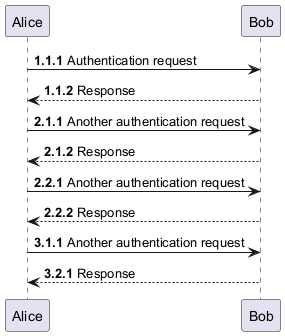
\includegraphics[scale=0.60]{imgw/img-3dac4e03bb423dab957803c7b32e00e1.png}
\end{center}




You can also use the value of \texttt{autonumber} with the \texttt{\%autonumber\%} variable:
\begin{verbatim}
@startuml
autonumber 10
Alice -> Bob
note right
  the <U+0025>autonumber<U+0025> works everywhere.
  Here, its value is ** %autonumber% **
end note
Bob --> Alice: //This is the response %autonumber%//
@enduml
\end{verbatim}
% true imgw/img-c76b3f88f668a16c13d51dc9c439b1a1.png
\begin{center}
% image width = 462
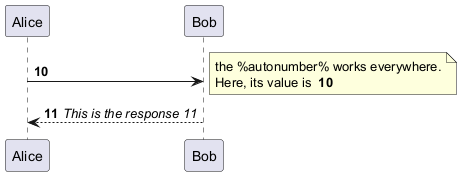
\includegraphics[scale=0.60]{imgw/img-c76b3f88f668a16c13d51dc9c439b1a1.png}
\end{center}
\textit{[Ref. QA-7119]}
%
% Page Title, Header and Footer
%
\subsection{Page Title, Header and Footer}


The \texttt{title} keyword is used to add a title to the page.


Pages can display headers and footers using \texttt{header} and \texttt{footer}.


\begin{verbatim}
@startuml

header Page Header
footer Page %page% of %lastpage%

title Example Title

Alice -> Bob : message 1
Alice -> Bob : message 2

@enduml
\end{verbatim}
% true imgw/img-8f5f426c37a97e11683b8ff09dcdef7b.png
\begin{center}
% image width = 145
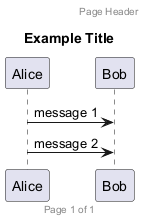
\includegraphics[scale=0.60]{imgw/img-8f5f426c37a97e11683b8ff09dcdef7b.png}
\end{center}




%
% Splitting diagrams
%
\subsection{Splitting diagrams}




The \texttt{newpage} keyword is used to split a diagram into several images.


You can put a title for the new page just after the \texttt{newpage}
keyword.  This title overrides the previously specified title if any.


This is very handy with \textit{Word} to print long diagram on
several pages.


(Note: this really does work.  Only the first page is shown below, but it is a display artifact.)


\begin{verbatim}
@startuml

Alice -> Bob : message 1
Alice -> Bob : message 2

newpage

Alice -> Bob : message 3
Alice -> Bob : message 4

newpage A title for the\nlast page

Alice -> Bob : message 5
Alice -> Bob : message 6
@enduml
\end{verbatim}
% true imgw/img-7e4b767bed83a15e2ac03000a10fa162.png
\begin{center}
% image width = 145
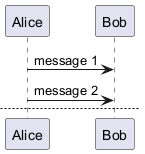
\includegraphics[scale=0.60]{imgw/img-7e4b767bed83a15e2ac03000a10fa162.png}
\end{center}


%
% Grouping message
%
\subsection{Grouping message}




It is possible to group messages together using the following
keywords:
\begin{itemize}
\item \texttt{alt/else}
\item \texttt{opt}
\item \texttt{loop}
\item \texttt{par}
\item \texttt{break}
\item \texttt{critical}
\item \texttt{group}, followed by a text to be displayed
\end{itemize}




It is possible to add a text that will be displayed into the
header (for \texttt{group}, see next paragraph \textit{'Secondary group label'}).


The \texttt{end} keyword is used to close the group.


Note that it is possible to nest groups.


\begin{verbatim}
@startuml
Alice -> Bob: Authentication Request

alt successful case

    Bob -> Alice: Authentication Accepted

else some kind of failure

    Bob -> Alice: Authentication Failure
    group My own label
    Alice -> Log : Log attack start
        loop 1000 times
            Alice -> Bob: DNS Attack
        end
    Alice -> Log : Log attack end
    end

else Another type of failure

   Bob -> Alice: Please repeat

end
@enduml
\end{verbatim}
% true imgw/img-4847318c167e0cda09263d390a6c3dd5.png
\begin{center}
% image width = 319
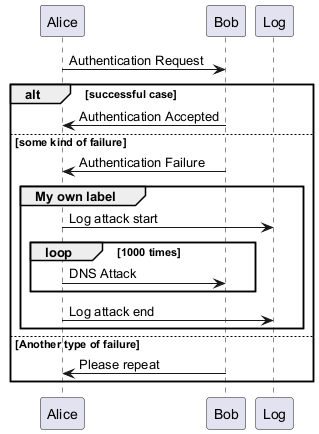
\includegraphics[scale=0.60]{imgw/img-4847318c167e0cda09263d390a6c3dd5.png}
\end{center}
%
% Secondary group label
%
\subsection{Secondary group label}


For \texttt{group}, it is possible to add, between\texttt{[} and \texttt{]}, a secondary text or label that will be displayed into the header.


\begin{verbatim}
@startuml
Alice -> Bob: Authentication Request
Bob -> Alice: Authentication Failure
group My own label [My own label 2]
    Alice -> Log : Log attack start
    loop 1000 times
        Alice -> Bob: DNS Attack
    end
    Alice -> Log : Log attack end
end
@enduml
\end{verbatim}
% true imgw/img-5af95ec979995fb20ab14e22575e99c2.png
\begin{center}
% image width = 292
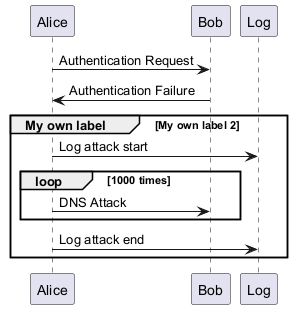
\includegraphics[scale=0.60]{imgw/img-5af95ec979995fb20ab14e22575e99c2.png}
\end{center}


\textit{[Ref. QA-2503]}
%
% Notes on messages
%
\subsection{Notes on messages}


It is possible to put notes on message using the \texttt{note left}
or \texttt{note right} keywords \textit{just after the message}.


You can have a multi-line note using the \texttt{end note}
keywords.


\begin{verbatim}
@startuml
Alice->Bob : hello
note left: this is a first note

Bob->Alice : ok
note right: this is another note

Bob->Bob : I am thinking
note left
a note
can also be defined
on several lines
end note
@enduml
\end{verbatim}
% true imgw/img-fb83d0b13cee295e367a6909b5c8ac34.png
\begin{center}
% image width = 320
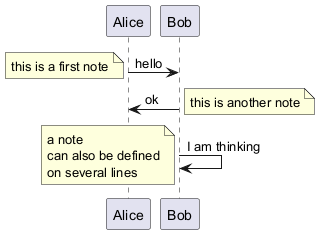
\includegraphics[scale=0.60]{imgw/img-fb83d0b13cee295e367a6909b5c8ac34.png}
\end{center}


%
% Some other notes
%
\subsection{Some other notes}




It is also possible to place notes relative to participant with \texttt{note left of} , \texttt{note right of} or \texttt{note over} keywords.


It is possible to highlight a note by changing its background color.


You can also have a multi-line note using the \texttt{end note} keywords.


\begin{verbatim}
@startuml
participant Alice
participant Bob
note left of Alice #aqua
This is displayed
left of Alice.
end note

note right of Alice: This is displayed right of Alice.

note over Alice: This is displayed over Alice.

note over Alice, Bob #FFAAAA: This is displayed\n over Bob and Alice.

note over Bob, Alice
This is yet another
example of
a long note.
end note
@enduml
\end{verbatim}
% true imgw/img-8d28b8bce9277dedab7ab65127d40e69.png
\begin{center}
% image width = 332
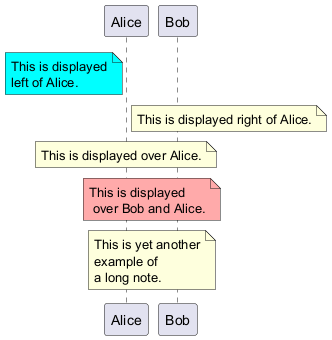
\includegraphics[scale=0.60]{imgw/img-8d28b8bce9277dedab7ab65127d40e69.png}
\end{center}
%
% Changing notes shape [hnote, rnote]
%
\subsection{Changing notes shape [hnote, rnote]}


You can use \texttt{hnote} and \texttt{rnote} keywords
to change note shapes :
\begin{itemize}
\item \texttt{hnote} for hexagonal note;
\item \texttt{rnote} for rectangle note.
\end{itemize}
\begin{verbatim}
@startuml
caller -> server : conReq
hnote over caller : idle
caller <- server : conConf
rnote over server
 "r" as rectangle
 "h" as hexagon
endrnote
rnote over server
 this is
 on several
 lines
endrnote
hnote over caller
 this is
 on several
 lines
endhnote
@enduml
\end{verbatim}
% true imgw/img-7833125523a0fcee5620f6712c551617.png
\begin{center}
% image width = 171
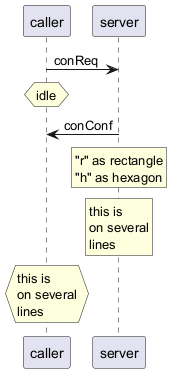
\includegraphics[scale=0.60]{imgw/img-7833125523a0fcee5620f6712c551617.png}
\end{center}


\textit{[Ref. QA-1765]}
%
% Note over all participants [across]
%
\subsection{Note over all participants [across]}


You can directly make a note over all participants, with the syntax:
\begin{itemize}
\item \texttt{note across: note\textunderscore description}
\end{itemize}


\begin{verbatim}
@startuml
Alice->Bob:m1
Bob->Charlie:m2
note over Alice, Charlie: Old method for note over all part. with:\n ""note over //FirstPart, LastPart//"".
note across: New method with:\n""note across""
Bob->Alice
hnote across:Note across all part.
@enduml
\end{verbatim}
% true imgw/img-06ba9ed80c25750c91cf7f5ebad81434.png
\begin{center}
% image width = 265
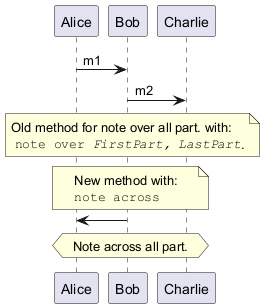
\includegraphics[scale=0.60]{imgw/img-06ba9ed80c25750c91cf7f5ebad81434.png}
\end{center}


\textit{[Ref. QA-9738]}
%
% Several notes aligned at the same level [/]
%
\subsection{Several notes aligned at the same level [/]}


You can make several notes aligned at the same level, with the syntax \texttt{/}:
\begin{itemize}
\item without \texttt{/} \textit{(by default, the notes are not aligned)}
\end{itemize}
\begin{verbatim}
@startuml
note over Alice : initial state of Alice
note over Bob : initial state of Bob
Bob -> Alice : hello
@enduml
\end{verbatim}
% true imgw/img-2d20b688283815c9941a1434b59d956d.png
\begin{center}
% image width = 187
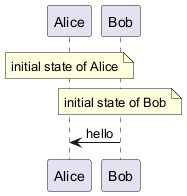
\includegraphics[scale=0.60]{imgw/img-2d20b688283815c9941a1434b59d956d.png}
\end{center}


\begin{itemize}
\item with \texttt{/} \textit{(the notes are aligned)}
\end{itemize}
\begin{verbatim}
@startuml
note over Alice : initial state of Alice
/ note over Bob : initial state of Bob
Bob -> Alice : hello
@enduml
\end{verbatim}
% true imgw/img-a5567ee92f01756037e83c2b6fe4c8e1.png
\begin{center}
% image width = 272
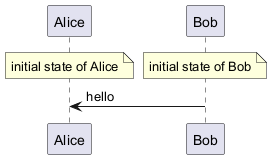
\includegraphics[scale=0.60]{imgw/img-a5567ee92f01756037e83c2b6fe4c8e1.png}
\end{center}


\textit{[Ref. QA-354]}
%
% Creole and HTML
%
\subsection{Creole and HTML}


It is also possible to use creole formatting:


\begin{verbatim}
@startuml
participant Alice
participant "The **Famous** Bob" as Bob

Alice -> Bob : hello --there--
... Some ~~long delay~~ ...
Bob -> Alice : ok
note left
  This is **bold**
  This is //italics//
  This is ""monospaced""
  This is --stroked--
  This is __underlined__
  This is ~~waved~~
end note

Alice -> Bob : A //well formatted// message
note right of Alice
 This is <back:cadetblue><size:18>displayed</size></back>
 __left of__ Alice.
end note
note left of Bob
 <u:red>This</u> is <color #118888>displayed</color>
 **<color purple>left of</color> <s:red>Alice</strike> Bob**.
end note
note over Alice, Bob
 <w:#FF33FF>This is hosted</w> by <img sourceforge.jpg>
end note
@enduml
\end{verbatim}
% true imgw/img-b29fecf37e95604e3ca76b3f9a0183e8.png
\begin{center}
% image width = 390
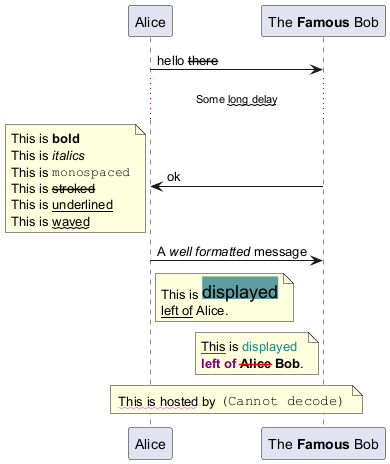
\includegraphics[scale=0.60]{imgw/img-b29fecf37e95604e3ca76b3f9a0183e8.png}
\end{center}


%
% Divider or separator
%
\subsection{Divider or separator}




If you want, you can split a diagram using \texttt{==} separator to
divide your diagram into logical steps.
\begin{verbatim}
@startuml

== Initialization ==

Alice -> Bob: Authentication Request
Bob --> Alice: Authentication Response

== Repetition ==

Alice -> Bob: Another authentication Request
Alice <-- Bob: another authentication Response

@enduml
\end{verbatim}
% true imgw/img-489093ed38f02901819aa16c789e1c5e.png
\begin{center}
% image width = 272
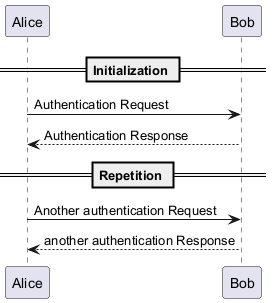
\includegraphics[scale=0.60]{imgw/img-489093ed38f02901819aa16c789e1c5e.png}
\end{center}
%
% Reference
%
\subsection{Reference}


You can use reference in a diagram, using the keyword \texttt{ref over}.
\begin{verbatim}
@startuml
participant Alice
actor Bob

ref over Alice, Bob : init

Alice -> Bob : hello

ref over Bob
  This can be on
  several lines
end ref
@enduml
\end{verbatim}
% true imgw/img-659ade911a29deec1f9f7f00fcf241ee.png
\begin{center}
% image width = 151
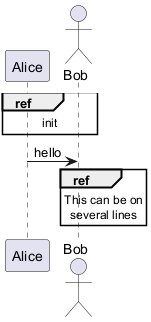
\includegraphics[scale=0.60]{imgw/img-659ade911a29deec1f9f7f00fcf241ee.png}
\end{center}


%
% Delay
%
\subsection{Delay}


You can use \texttt{...} to indicate a delay in the diagram.
And it is also possible to put a message with this delay.
\begin{verbatim}
@startuml

Alice -> Bob: Authentication Request
...
Bob --> Alice: Authentication Response
...5 minutes later...
Bob --> Alice: Good Bye !

@enduml
\end{verbatim}
% true imgw/img-8d667df4fc22a9d08937418e51baeaf5.png
\begin{center}
% image width = 220
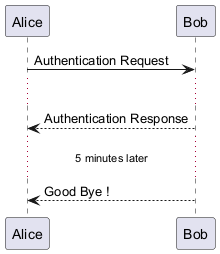
\includegraphics[scale=0.60]{imgw/img-8d667df4fc22a9d08937418e51baeaf5.png}
\end{center}
%
% Text wrapping
%
\subsection{Text wrapping}


To break long messages, you can manually add \texttt{\textbackslash n} in your text.


Another option is to use \texttt{maxMessageSize} setting:


\begin{verbatim}
@startuml
skinparam maxMessageSize 50
participant a
participant b
a -> b :this\nis\nmanually\ndone
a -> b :this is a very long message on several words
@enduml
\end{verbatim}
% true imgw/img-e1dfc5c0f251a2231037cc984b546a1b.png
\begin{center}
% image width = 108
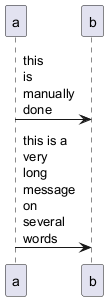
\includegraphics[scale=0.60]{imgw/img-e1dfc5c0f251a2231037cc984b546a1b.png}
\end{center}
%
% Space
%
\subsection{Space}




You can use \texttt{|||} to indicate some spacing in the diagram.


It is also possible to specify a number of pixel to be used.
\begin{verbatim}
@startuml

Alice -> Bob: message 1
Bob --> Alice: ok
|||
Alice -> Bob: message 2
Bob --> Alice: ok
||45||
Alice -> Bob: message 3
Bob --> Alice: ok

@enduml
\end{verbatim}
% true imgw/img-87f99d4e04d76ba558c014ff46a38f54.png
\begin{center}
% image width = 139
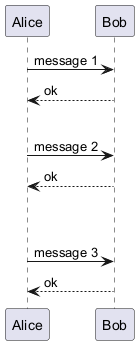
\includegraphics[scale=0.60]{imgw/img-87f99d4e04d76ba558c014ff46a38f54.png}
\end{center}


%
% Lifeline Activation and Destruction
%
\subsection{Lifeline Activation and Destruction}


The \texttt{activate} and \texttt{deactivate} are used to denote
participant activation.


Once a participant is activated, its lifeline appears.


The \texttt{activate} and \texttt{deactivate} apply on
the previous message.


The \texttt{destroy} denote the end of the lifeline of a
participant.


\begin{verbatim}
@startuml
participant User

User -> A: DoWork
activate A

A -> B: << createRequest >>
activate B

B -> C: DoWork
activate C
C --> B: WorkDone
destroy C

B --> A: RequestCreated
deactivate B

A -> User: Done
deactivate A

@enduml
\end{verbatim}
% true imgw/img-b0041b383b98de46cd8d933a7be82e9c.png
\begin{center}
% image width = 338
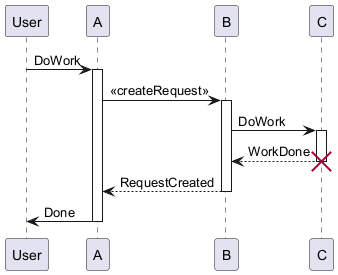
\includegraphics[scale=0.60]{imgw/img-b0041b383b98de46cd8d933a7be82e9c.png}
\end{center}




Nested lifeline can be used, and it is possible to add a color on the lifeline.


\begin{verbatim}
@startuml
participant User

User -> A: DoWork
activate A #FFBBBB

A -> A: Internal call
activate A #DarkSalmon

A -> B: << createRequest >>
activate B

B --> A: RequestCreated
deactivate B
deactivate A
A -> User: Done
deactivate A

@enduml
\end{verbatim}
% true imgw/img-6fd48effdebe01edcbaff4c8d18fbdc3.png
\begin{center}
% image width = 248
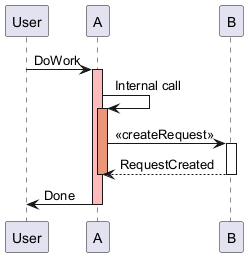
\includegraphics[scale=0.60]{imgw/img-6fd48effdebe01edcbaff4c8d18fbdc3.png}
\end{center}


Autoactivation is possible and works with the return keywords:


\begin{verbatim}
@startuml
autoactivate on
alice -> bob : hello
bob -> bob : self call
bill -> bob #005500 : hello from thread 2
bob -> george ** : create
return done in thread 2
return rc
bob -> george !! : delete
return success

@enduml
\end{verbatim}
% true imgw/img-7b885e37c75d99046f1aa7a4898b3993.png
\begin{center}
% image width = 332
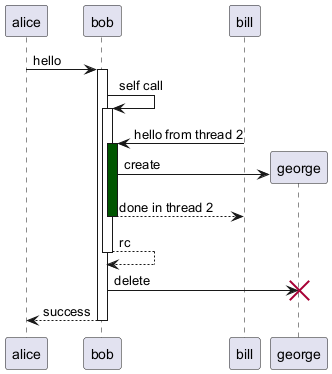
\includegraphics[scale=0.60]{imgw/img-7b885e37c75d99046f1aa7a4898b3993.png}
\end{center}
%
% Return
%
\subsection{Return}


Command \texttt{return} generates a return message with optional text label.


The return point is that which caused the most recent life-line activation.


The syntax is \texttt{return label} where \texttt{label} if provided is any string acceptable for conventional messages.




\begin{verbatim}
@startuml
Bob -> Alice : hello
activate Alice
Alice -> Alice : some action
return bye
@enduml
\end{verbatim}
% true imgw/img-7d491cd723e8d6f752bd0f45b9cf763b.png
\begin{center}
% image width = 164
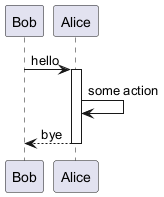
\includegraphics[scale=0.60]{imgw/img-7d491cd723e8d6f752bd0f45b9cf763b.png}
\end{center}


%
% Participant creation
%
\subsection{Participant creation}




You can use the \texttt{create} keyword just before the first
reception of a message to emphasize the fact that this message is
actually \textit{creating} this new object.
\begin{verbatim}
@startuml
Bob -> Alice : hello

create Other
Alice -> Other : new

create control String
Alice -> String
note right : You can also put notes!

Alice --> Bob : ok

@enduml
\end{verbatim}
% true imgw/img-5c1f3d97532da20d20cd4121e47f612a.png
\begin{center}
% image width = 392
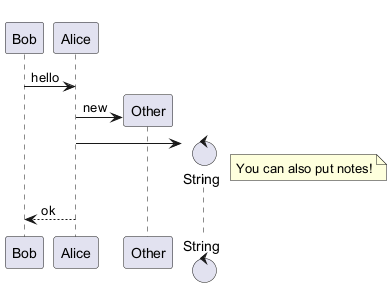
\includegraphics[scale=0.60]{imgw/img-5c1f3d97532da20d20cd4121e47f612a.png}
\end{center}


%
% Shortcut syntax for activation, deactivation, creation
%
\subsection{Shortcut syntax for activation, deactivation, creation}




Immediately after specifying the target participant, the following syntax can be used:


\begin{itemize}
\item \texttt{++} Activate the target (optionally a color may follow this)
\item \texttt{--} Deactivate the source
\item \texttt{**} Create an instance of the target
\item \texttt{!!} Destroy an instance of the target
\end{itemize}


\begin{verbatim}
@startuml
alice -> bob ++ : hello
bob -> bob ++ : self call
bob -> bib ++  #005500 : hello
bob -> george ** : create
return done
return rc
bob -> george !! : delete
return success
@enduml
\end{verbatim}
% true imgw/img-18d920168f7f8816c053fdaa158b7a38.png
\begin{center}
% image width = 271
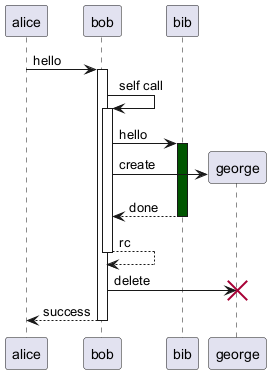
\includegraphics[scale=0.60]{imgw/img-18d920168f7f8816c053fdaa158b7a38.png}
\end{center}


Then you can mix activation and deactivation, on same line:
\begin{verbatim}
@startuml
alice   ->  bob     ++   : hello1
bob     ->  charlie --++ : hello2
charlie --> alice   --   : ok
@enduml
\end{verbatim}
% true imgw/img-524410099bd22fe6c46a82ea48c3a016.png
\begin{center}
% image width = 181
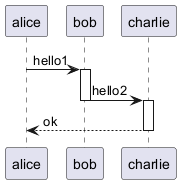
\includegraphics[scale=0.60]{imgw/img-524410099bd22fe6c46a82ea48c3a016.png}
\end{center}


\begin{verbatim}
@startuml
@startuml
alice -> bob   --++ #gold: hello
bob   -> alice --++ #gold: you too
alice -> bob   --: step1
alice -> bob   : step2
@enduml
@enduml
\end{verbatim}
% true imgw/img-5fce03de23461ed26a1508bc3f77ff5f.png
\begin{center}
% image width = 121
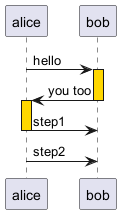
\includegraphics[scale=0.60]{imgw/img-5fce03de23461ed26a1508bc3f77ff5f.png}
\end{center}


\textit{[Ref. QA-4834, QA-9573 and QA-13234]}
%
% Incoming and outgoing messages
%
\subsection{Incoming and outgoing messages}


You can use incoming or outgoing arrows if you want to focus on a part
of the diagram.


Use square brackets to denote the left "\texttt{[}" or the
right "\texttt{]}" side of the diagram.
\begin{verbatim}
@startuml
[-> A: DoWork

activate A

A -> A: Internal call
activate A

A ->] : << createRequest >>

A<--] : RequestCreated
deactivate A
[<- A: Done
deactivate A
@enduml
\end{verbatim}
% true imgw/img-63fc04692eb5b25a273398ea3077ef76.png
\begin{center}
% image width = 208
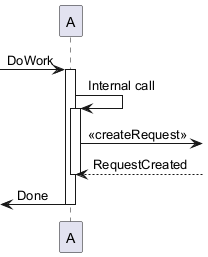
\includegraphics[scale=0.60]{imgw/img-63fc04692eb5b25a273398ea3077ef76.png}
\end{center}




You can also have the following syntax:
\begin{verbatim}
@startuml
participant Alice
participant Bob #lightblue
Alice -> Bob
Bob -> Carol
...
[-> Bob
[o-> Bob
[o->o Bob
[x-> Bob
...
[<- Bob
[x<- Bob
...
Bob ->]
Bob ->o]
Bob o->o]
Bob ->x]
...
Bob <-]
Bob x<-]

@enduml
\end{verbatim}
% true imgw/img-84e349d9dfdb4f5a65542aa3fd68e374.png
\begin{center}
% image width = 165
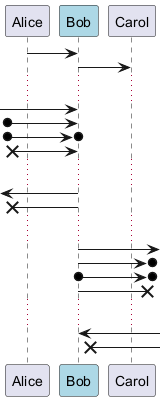
\includegraphics[scale=0.60]{imgw/img-84e349d9dfdb4f5a65542aa3fd68e374.png}
\end{center}
%
% Short arrows for incoming and outgoing messages
%
\subsection{Short arrows for incoming and outgoing messages}


You can have \textbf{short} arrows with using \texttt{?}.


\begin{verbatim}
@startuml
?-> Alice    : ""?->""\n**short** to actor1
[-> Alice    : ""[->""\n**from start** to actor1
[-> Bob      : ""[->""\n**from start** to actor2
?-> Bob      : ""?->""\n**short** to actor2
Alice ->]    : ""->]""\nfrom actor1 **to end**
Alice ->?    : ""->?""\n**short** from actor1
Alice -> Bob : ""->"" \nfrom actor1 to actor2
@enduml
\end{verbatim}
% true imgw/img-b9cde1bd1c7484ac43dcc31caa2b86d3.png
\begin{center}
% image width = 307
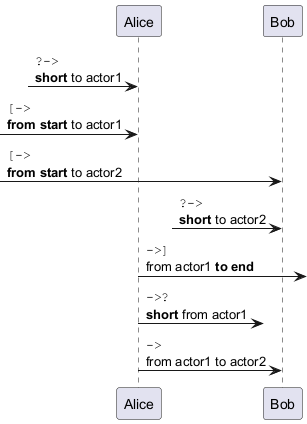
\includegraphics[scale=0.60]{imgw/img-b9cde1bd1c7484ac43dcc31caa2b86d3.png}
\end{center}


\textit{[Ref. QA-310]}
%
% Anchors and Duration
%
\subsection{Anchors and Duration}






With \texttt{teoz} it is possible to add anchors to the diagram and use the anchors to specify duration time.
\begin{verbatim}
@startuml
!pragma teoz true

{start} Alice -> Bob : start doing things during duration
Bob -> Max : something
Max -> Bob : something else
{end} Bob -> Alice : finish

{start} <-> {end} : some time

@enduml
\end{verbatim}
% true imgw/img-7fc708ff224c1ee3cb9607fb647c3e11.png
\begin{center}
% image width = 377
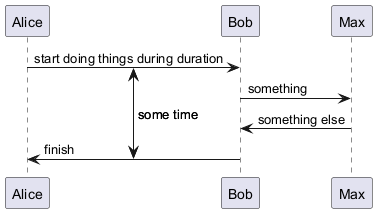
\includegraphics[scale=0.60]{imgw/img-7fc708ff224c1ee3cb9607fb647c3e11.png}
\end{center}


You can use the \texttt{-P} command-line option to specify the pragma:
\begin{verbatim}
java -jar plantuml.jar -Pteoz=true
\end{verbatim}
\textit{[Ref. issue-582]}
%
% Stereotypes and Spots
%
\subsection{Stereotypes and Spots}






It is possible to add stereotypes to participants using \texttt{<<}
and \texttt{>>}.


In the stereotype, you can add a spotted character
in a colored circle using the syntax \texttt{(X,color)}.
\begin{verbatim}
@startuml

participant "Famous Bob" as Bob << Generated >>
participant Alice << (C,#ADD1B2) Testable >>

Bob->Alice: First message

@enduml
\end{verbatim}
% true imgw/img-9c89f6d111ffba9a5b4e94902a65a286.png
\begin{center}
% image width = 226
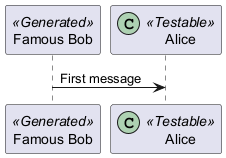
\includegraphics[scale=0.60]{imgw/img-9c89f6d111ffba9a5b4e94902a65a286.png}
\end{center}


By default, the \textit{guillemet} character is used to display the stereotype.
You can change this behavious using the skinparam \texttt{guillemet}:


\begin{verbatim}
@startuml

skinparam guillemet false
participant "Famous Bob" as Bob << Generated >>
participant Alice << (C,#ADD1B2) Testable >>

Bob->Alice: First message

@enduml
\end{verbatim}
% true imgw/img-a633b72a8cfb3d3857dff8c7a4d07ae1.png
\begin{center}
% image width = 276
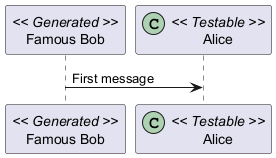
\includegraphics[scale=0.60]{imgw/img-a633b72a8cfb3d3857dff8c7a4d07ae1.png}
\end{center}


\begin{verbatim}
@startuml

participant Bob << (C,#ADD1B2) >>
participant Alice << (C,#ADD1B2) >>

Bob->Alice: First message

@enduml
\end{verbatim}
% true imgw/img-fcbe3a70f6c0dd0055400b8529d4ccc3.png
\begin{center}
% image width = 185
\includegraphics[scale=0.60]{imgw/img-fcbe3a70f6c0dd0055400b8529d4ccc3.png}
\end{center}


%
% Position of the stereotypes
%
\subsection{Position of the stereotypes}


It is possible to define stereotypes position (\texttt{top} or \texttt{bottom}) with the command \texttt{skinparam stereotypePosition}.


\subsubsection{Top postion \textit{(by default)}}
\begin{verbatim}
@startuml
skinparam stereotypePosition top

participant A<<st1>>
participant B<<st2>>
A --> B : stereo test
@enduml
\end{verbatim}
% true imgw/img-577bd0705f25270e47361949c653baa9.png
\begin{center}
% image width = 142
\includegraphics[scale=0.60]{imgw/img-577bd0705f25270e47361949c653baa9.png}
\end{center}


\subsubsection{Bottom postion}
\begin{verbatim}
@startuml
skinparam stereotypePosition bottom

participant A<<st1>>
participant B<<st2>>
A --> B : stereo test
@enduml
\end{verbatim}
% true imgw/img-dd969edfbd5e760b6b839d17d649de4c.png
\begin{center}
% image width = 142
\includegraphics[scale=0.60]{imgw/img-dd969edfbd5e760b6b839d17d649de4c.png}
\end{center}


\textit{[Ref. QA-18650]}
%
% More information on titles
%
\subsection{More information on titles}


You can use creole formatting in the title.


\begin{verbatim}
@startuml

title __Simple__ **communication** example

Alice -> Bob: Authentication Request
Bob -> Alice: Authentication Response

@enduml
\end{verbatim}
% true imgw/img-1121d5f5f9130f0ff9a0abdafbad0bcd.png
\begin{center}
% image width = 240
\includegraphics[scale=0.60]{imgw/img-1121d5f5f9130f0ff9a0abdafbad0bcd.png}
\end{center}
You can add newline using \texttt{\textbackslash n} in the title description.
\begin{verbatim}
@startuml

title __Simple__ communication example\non several lines

Alice -> Bob: Authentication Request
Bob -> Alice: Authentication Response

@enduml
\end{verbatim}
% true imgw/img-79979f5af15b77af1d0985c873b87ebe.png
\begin{center}
% image width = 240
\includegraphics[scale=0.60]{imgw/img-79979f5af15b77af1d0985c873b87ebe.png}
\end{center}
You can also define title on several lines using \texttt{title}
and \texttt{end title} keywords.
\begin{verbatim}
@startuml

title
 <u>Simple</u> communication example
 on <i>several</i> lines and using <font color=red>html</font>
 This is hosted by <img:sourceforge.jpg>
end title

Alice -> Bob: Authentication Request
Bob -> Alice: Authentication Response

@enduml
\end{verbatim}
% true imgw/img-bb6bfad36009c3e767dc81565a6282a5.png
\begin{center}
% image width = 271
\includegraphics[scale=0.60]{imgw/img-bb6bfad36009c3e767dc81565a6282a5.png}
\end{center}


%
% Participants encompass
%
\subsection{Participants encompass}






It is possible to draw a box around some participants, using \texttt{box}
and \texttt{end box} commands.


You can add an optional title or a
optional background color, after the \texttt{box} keyword.


\begin{verbatim}
@startuml

box "Internal Service" #LightBlue
participant Bob
participant Alice
end box
participant Other

Bob -> Alice : hello
Alice -> Other : hello

@enduml
\end{verbatim}
% true imgw/img-01481d782566c715e3d44cdfbba2e73d.png
\begin{center}
% image width = 163
\includegraphics[scale=0.60]{imgw/img-01481d782566c715e3d44cdfbba2e73d.png}
\end{center}




It is also possible to nest boxes - to draw a box within a box - when using the teoz rendering engine, for example:


\begin{verbatim}
@startuml

!pragma teoz true
box "Internal Service" #LightBlue
participant Bob
box "Subteam"
participant Alice
participant John
end box

end box
participant Other

Bob -> Alice : hello
Alice -> John : hello
John -> Other: Hello

@enduml
\end{verbatim}
% true imgw/img-4d54316b38eb7af9b457a6c1fcb6e987.png
\begin{center}
% image width = 236
\includegraphics[scale=0.60]{imgw/img-4d54316b38eb7af9b457a6c1fcb6e987.png}
\end{center}
%
% Removing Foot Boxes
%
\subsection{Removing Foot Boxes}


You can use the \texttt{hide footbox} keywords to remove the foot boxes
of the diagram.


\begin{verbatim}
@startuml

hide footbox
title Foot Box removed

Alice -> Bob: Authentication Request
Bob --> Alice: Authentication Response

@enduml
\end{verbatim}
% true imgw/img-494dcebcd04c6f6922dd00c09d52f8b5.png
\begin{center}
% image width = 220
\includegraphics[scale=0.60]{imgw/img-494dcebcd04c6f6922dd00c09d52f8b5.png}
\end{center}


%
% Skinparam
%
\subsection{Skinparam}




You can use the skinparam
command to change colors and fonts for the drawing.




You can use this command:
\begin{itemize}
\item In the diagram definition, like any other commands,
\item In an included file,
\item In a configuration file, provided in the command line or the ANT task.
\end{itemize}


You can also change other rendering parameter, as seen in the following examples:


\begin{verbatim}
@startuml
skinparam sequenceArrowThickness 2
skinparam roundcorner 20
skinparam maxmessagesize 60
skinparam sequenceParticipant underline

actor User
participant "First Class" as A
participant "Second Class" as B
participant "Last Class" as C

User -> A: DoWork
activate A

A -> B: Create Request
activate B

B -> C: DoWork
activate C
C --> B: WorkDone
destroy C

B --> A: Request Created
deactivate B

A --> User: Done
deactivate A

@enduml
\end{verbatim}
% true imgw/img-2ac222a5f0868a3e370e7271c766e034.png
\begin{center}
% image width = 338
\includegraphics[scale=0.60]{imgw/img-2ac222a5f0868a3e370e7271c766e034.png}
\end{center}


\begin{verbatim}
@startuml
skinparam backgroundColor #EEEBDC
skinparam handwritten true

skinparam sequence {
ArrowColor DeepSkyBlue
ActorBorderColor DeepSkyBlue
LifeLineBorderColor blue
LifeLineBackgroundColor #A9DCDF

ParticipantBorderColor DeepSkyBlue
ParticipantBackgroundColor DodgerBlue
ParticipantFontName Impact
ParticipantFontSize 17
ParticipantFontColor #A9DCDF

ActorBackgroundColor aqua
ActorFontColor DeepSkyBlue
ActorFontSize 17
ActorFontName Aapex
}

actor User
participant "First Class" as A
participant "Second Class" as B
participant "Last Class" as C

User -> A: DoWork
activate A

A -> B: Create Request
activate B

B -> C: DoWork
activate C
C --> B: WorkDone
destroy C

B --> A: Request Created
deactivate B

A --> User: Done
deactivate A

@enduml
\end{verbatim}
% true imgw/img-9d207922fcde3e2dc4a7fe944f883b38.png
\begin{center}
% image width = 385
\includegraphics[scale=0.60]{imgw/img-9d207922fcde3e2dc4a7fe944f883b38.png}
\end{center}




%
% Changing padding
%
\subsection{Changing padding}




It is possible to tune some padding settings.


\begin{verbatim}
@startuml
skinparam ParticipantPadding 20
skinparam BoxPadding 10

box "Foo1"
participant Alice1
participant Alice2
end box
box "Foo2"
participant Bob1
participant Bob2
end box
Alice1 -> Bob1 : hello
Alice1 -> Out : out
@enduml
\end{verbatim}
% true imgw/img-f615013811d01bf754d534fd0543e550.png
\begin{center}
% image width = 504
\includegraphics[scale=0.60]{imgw/img-f615013811d01bf754d534fd0543e550.png}
\end{center}




%
% Appendix: Examples of all arrow type
%
\subsection{Appendix: Examples of all arrow type}


\subsubsection{Normal arrow}
\begin{verbatim}
@startuml
participant Alice as a
participant Bob   as b
a ->     b : ""->   ""
a ->>    b : ""->>  ""
a -\     b : ""-\   ""
a -\\    b : ""-\\\\""
a -/     b : ""-/   ""
a -//    b : ""-//  ""
a ->x    b : ""->x  ""
a x->    b : ""x->  ""
a o->    b : ""o->  ""
a ->o    b : ""->o  ""
a o->o   b : ""o->o ""
a <->    b : ""<->  ""
a o<->o  b : ""o<->o""
a x<->x  b : ""x<->x""
a ->>o   b : ""->>o ""
a -\o    b : ""-\o  ""
a -\\o   b : ""-\\\\o""
a -/o    b : ""-/o  ""
a -//o   b : ""-//o ""
a x->o   b : ""x->o ""
@enduml
\end{verbatim}
% true imgw/img-a14004de730c5a460d924597e0da9115.png
\begin{center}
% image width = 114
\includegraphics[scale=0.60]{imgw/img-a14004de730c5a460d924597e0da9115.png}
\end{center}


\subsubsection{Itself arrow}
\begin{verbatim}
@startuml
participant Alice as a
participant Bob   as b
a ->     a : ""->   ""
a ->>    a : ""->>  ""
a -\     a : ""-\   ""
a -\\    a : ""-\\\\""
a -/     a : ""-/   ""
a -//    a : ""-//  ""
a ->x    a : ""->x  ""
a x->    a : ""x->  ""
a o->    a : ""o->  ""
a ->o    a : ""->o  ""
a o->o   a : ""o->o ""
a <->    a : ""<->  ""
a o<->o  a : ""o<->o""
a x<->x  a : ""x<->x""
a ->>o   a : ""->>o ""
a -\o    a : ""-\o  ""
a -\\o   a : ""-\\\\o""
a -/o    a : ""-/o  ""
a -//o   a : ""-//o ""
a x->o   a : ""x->o ""
@enduml
\end{verbatim}
% true imgw/img-8236cd98b4731207bf5b3bcffe83cc00.png
\begin{center}
% image width = 104
\includegraphics[scale=0.60]{imgw/img-8236cd98b4731207bf5b3bcffe83cc00.png}
\end{center}


\subsubsection{Incoming and outgoing messages (with '[', ']')}
\subsubsection{Incoming messages (with '[')}
\begin{verbatim}
@startuml
participant Alice as a
participant Bob   as b
[->      b : ""[->   ""
[->>     b : ""[->>  ""
[-\      b : ""[-\   ""
[-\\     b : ""[-\\\\""
[-/      b : ""[-/   ""
[-//     b : ""[-//  ""
[->x     b : ""[->x  ""
[x->     b : ""[x->  ""
[o->     b : ""[o->  ""
[->o     b : ""[->o  ""
[o->o    b : ""[o->o ""
[<->     b : ""[<->  ""
[o<->o   b : ""[o<->o""
[x<->x   b : ""[x<->x""
[->>o    b : ""[->>o ""
[-\o     b : ""[-\o  ""
[-\\o    b : ""[-\\\\o""
[-/o     b : ""[-/o  ""
[-//o    b : ""[-//o ""
[x->o    b : ""[x->o ""
@enduml
\end{verbatim}
% true imgw/img-7caa8cc5c1a88bd5587a265356105cd8.png
\begin{center}
% image width = 103
\includegraphics[scale=0.60]{imgw/img-7caa8cc5c1a88bd5587a265356105cd8.png}
\end{center}


\subsubsection{Outgoing messages (with ']')}
\begin{verbatim}
@startuml
participant Alice as a
participant Bob   as b
a ->]      : ""->]   ""
a ->>]     : ""->>]  ""
a -\]      : ""-\]   ""
a -\\]     : ""-\\\\]""
a -/]      : ""-/]   ""
a -//]     : ""-//]  ""
a ->x]     : ""->x]  ""
a x->]     : ""x->]  ""
a o->]     : ""o->]  ""
a ->o]     : ""->o]  ""
a o->o]    : ""o->o] ""
a <->]     : ""<->]  ""
a o<->o]   : ""o<->o]""
a x<->x]   : ""x<->x]""
a ->>o]    : ""->>o] ""
a -\o]     : ""-\o]  ""
a -\\o]    : ""-\\\\o]""
a -/o]     : ""-/o]  ""
a -//o]    : ""-//o] ""
a x->o]    : ""x->o] ""
@enduml
\end{verbatim}
% true imgw/img-2158c64e14946b6b276a06085e4a8a37.png
\begin{center}
% image width = 110
\includegraphics[scale=0.60]{imgw/img-2158c64e14946b6b276a06085e4a8a37.png}
\end{center}


\subsubsection{Short incoming and outgoing messages (with '?')}
\subsubsection{Short incoming (with '?')}
\begin{verbatim}
@startuml
participant Alice as a
participant Bob   as b
a ->     b : //Long long label//
?->      b : ""?->   ""
?->>     b : ""?->>  ""
?-\      b : ""?-\   ""
?-\\     b : ""?-\\\\""
?-/      b : ""?-/   ""
?-//     b : ""?-//  ""
?->x     b : ""?->x  ""
?x->     b : ""?x->  ""
?o->     b : ""?o->  ""
?->o     b : ""?->o  ""
?o->o    b : ""?o->o ""
?<->     b : ""?<->  ""
?o<->o   b : ""?o<->o""
?x<->x   b : ""?x<->x""
?->>o    b : ""?->>o ""
?-\o     b : ""?-\o  ""
?-\\o    b : ""?-\\\\o ""
?-/o     b : ""?-/o  ""
?-//o    b : ""?-//o ""
?x->o    b : ""?x->o ""
@enduml
\end{verbatim}
% true imgw/img-a69f4fcce82e8fa500e2a898194cffca.png
\begin{center}
% image width = 163
\includegraphics[scale=0.60]{imgw/img-a69f4fcce82e8fa500e2a898194cffca.png}
\end{center}


\subsubsection{Short outgoing (with '?')}
\begin{verbatim}
@startuml
participant Alice as a
participant Bob   as b
a ->     b : //Long long label//
a ->?      : ""->?   ""
a ->>?     : ""->>?  ""
a -\?      : ""-\?   ""
a -\\?     : ""-\\\\?""
a -/?      : ""-/?   ""
a -//?     : ""-//?  ""
a ->x?     : ""->x?  ""
a x->?     : ""x->?  ""
a o->?     : ""o->?  ""
a ->o?     : ""->o?  ""
a o->o?    : ""o->o? ""
a <->?     : ""<->?  ""
a o<->o?   : ""o<->o?""
a x<->x?   : ""x<->x?""
a ->>o?    : ""->>o? ""
a -\o?     : ""-\o?  ""
a -\\o?    : ""-\\\\o?""
a -/o?     : ""-/o?  ""
a -//o?    : ""-//o? ""
a x->o?    : ""x->o? ""
@enduml
\end{verbatim}
% true imgw/img-132305d4d41328d264093aaa08efb379.png
\begin{center}
% image width = 163
\includegraphics[scale=0.60]{imgw/img-132305d4d41328d264093aaa08efb379.png}
\end{center}
%
% Specific SkinParameter
%
\subsection{Specific SkinParameter}


\subsubsection{By default}
\begin{verbatim}
@startuml
Bob -> Alice : hello
Alice -> Bob : ok
@enduml
\end{verbatim}
% true imgw/img-81a4f72445c3c52b7cc56732406a1dc3.png
\begin{center}
% image width = 103
\includegraphics[scale=0.60]{imgw/img-81a4f72445c3c52b7cc56732406a1dc3.png}
\end{center}


\subsubsection{LifelineStrategy }


\begin{itemize}
\item nosolid \textit{(by default)}
\end{itemize}
\begin{verbatim}
@startuml
skinparam lifelineStrategy nosolid
Bob -> Alice : hello
Alice -> Bob : ok
@enduml
\end{verbatim}
% true imgw/img-0a0f41aa2176b75595f9e713f174827a.png
\begin{center}
% image width = 103
\includegraphics[scale=0.60]{imgw/img-0a0f41aa2176b75595f9e713f174827a.png}
\end{center}
\textit{[Ref. QA-9016]}


\begin{itemize}
\item solid
\end{itemize}
In order to have solid life line in sequence diagrams, you can use: \texttt{skinparam lifelineStrategy solid}
\begin{verbatim}
@startuml
skinparam lifelineStrategy solid
Bob -> Alice : hello
Alice -> Bob : ok
@enduml
\end{verbatim}
% true imgw/img-0e6c7e64383536bb363507f6f7cf7b8c.png
\begin{center}
% image width = 103
\includegraphics[scale=0.60]{imgw/img-0e6c7e64383536bb363507f6f7cf7b8c.png}
\end{center}


\textit{[Ref. QA-2794]}


\subsubsection{style strictuml}
To be conform to strict UML (\textit{for arrow style: emits triangle rather than sharp arrowheads}), you can use:
\begin{itemize}
\item \texttt{skinparam style strictuml}
\end{itemize}
\begin{verbatim}
@startuml
skinparam style strictuml
Bob -> Alice : hello
Alice -> Bob : ok
@enduml
\end{verbatim}
% true imgw/img-43c0624948a53d5fd55da6ba4b1d5369.png
\begin{center}
% image width = 103
\includegraphics[scale=0.60]{imgw/img-43c0624948a53d5fd55da6ba4b1d5369.png}
\end{center}
\textit{[Ref. QA-1047]}
%
% Hide unlinked participant
%
\subsection{Hide unlinked participant }


By default, all participants are displayed.
\begin{verbatim}
@startuml
participant Alice
participant Bob
participant Carol

Alice -> Bob : hello
@enduml
\end{verbatim}
% true imgw/img-72c891647a1c57f2b3dbff2dd4c4dd3d.png
\begin{center}
% image width = 160
\includegraphics[scale=0.60]{imgw/img-72c891647a1c57f2b3dbff2dd4c4dd3d.png}
\end{center}


But you can \texttt{hide unlinked} participant.
\begin{verbatim}
@startuml
hide unlinked
participant Alice
participant Bob
participant Carol

Alice -> Bob : hello
@enduml
\end{verbatim}
% true imgw/img-b4609c8640dca71bb65b86ae4a34c3d8.png
\begin{center}
% image width = 103
\includegraphics[scale=0.60]{imgw/img-b4609c8640dca71bb65b86ae4a34c3d8.png}
\end{center}




\textit{[Ref. QA-4247]}
%
% Color a group message
%
\subsection{Color a group message}




It is possible to color a group messages:


\begin{verbatim}
@startuml
Alice -> Bob: Authentication Request
alt#Gold #LightBlue Successful case
    Bob -> Alice: Authentication Accepted
else #Pink Failure
    Bob -> Alice: Authentication Rejected
end
@enduml
\end{verbatim}
% true imgw/img-2d3195fe252864acdfcf9cf8bc22d02e.png
\begin{center}
% image width = 241
\includegraphics[scale=0.60]{imgw/img-2d3195fe252864acdfcf9cf8bc22d02e.png}
\end{center}
\textit{[Ref. QA-4750 and QA-6410]}
%
% Mainframe
%
\subsection{Mainframe}


\begin{verbatim}
@startuml
mainframe This is a **mainframe**
Alice->Bob : Hello
@enduml
\end{verbatim}
% true imgw/img-74f1ac5f2491c99938f9ffb694d3baea.png
\begin{center}
% image width = 156
\includegraphics[scale=0.60]{imgw/img-74f1ac5f2491c99938f9ffb694d3baea.png}
\end{center}


\textit{[Ref. QA-4019 and Issue\#148]}
%
% Slanted or odd arrows
%
\subsection{Slanted or odd arrows }


You can use the \texttt{(nn)} option (before or after arrow) to make the arrows slanted, where \textit{nn} is the number of shift pixels.


\textit{[Available only after v1.2022.6beta+]}


\begin{verbatim}
@startuml
A ->(10) B: text 10
B ->(10) A: text 10

A ->(10) B: text 10
A (10)<- B: text 10
@enduml
\end{verbatim}
% true imgw/img-89644ab82cec13c65ff82e91309d4bf5.png
\begin{center}
% image width = 96
\includegraphics[scale=0.60]{imgw/img-89644ab82cec13c65ff82e91309d4bf5.png}
\end{center}


\begin{verbatim}
@startuml
A ->(40) B++: Rq
B -->(20) A--: Rs
@enduml
\end{verbatim}
% true imgw/img-d47da36df96c90f3d60a47954c47f642.png
\begin{center}
% image width = 78
\includegraphics[scale=0.60]{imgw/img-d47da36df96c90f3d60a47954c47f642.png}
\end{center}
\textit{[Ref. QA-14145]}


\begin{verbatim}
@startuml
!pragma teoz true
A ->(50) C: Starts\nwhen 'B' sends
& B ->(25) C: \nBut B's message\n arrives before A's
@enduml
\end{verbatim}
% true imgw/img-bb31618148ec36b7aca9b1947a4adec9.png
\begin{center}
% image width = 272
\includegraphics[scale=0.60]{imgw/img-bb31618148ec36b7aca9b1947a4adec9.png}
\end{center}
\textit{[Ref. QA-6684]}


\begin{verbatim}
@startuml
!pragma teoz true

S1 ->(30) S2: msg 1\n
& S2 ->(30) S1: msg 2

note left S1: msg\nS2 to S1
& note right S2: msg\nS1 to S2
@enduml
\end{verbatim}
% true imgw/img-8fd104e79e6b85b1345f9763b4b5881d.png
\begin{center}
% image width = 226
\includegraphics[scale=0.60]{imgw/img-8fd104e79e6b85b1345f9763b4b5881d.png}
\end{center}
\textit{[Ref. QA-1072]}
%
% Parallel messages __(with teoz)__
%
\subsection{Parallel messages \textit{(with teoz)}}


You can use the \texttt{\&} teoz command to display parallel messages:


\begin{verbatim}
@startuml
!pragma teoz true
Alice -> Bob : hello
& Bob -> Charlie : hi
@enduml
\end{verbatim}
% true imgw/img-7afe35deb2c3bad3cc064d53e7c264e8.png
\begin{center}
% image width = 171
\includegraphics[scale=0.60]{imgw/img-7afe35deb2c3bad3cc064d53e7c264e8.png}
\end{center}


\textit{(See also Teoz architecture)}

%\include{use-case-diagram}
%\include{class-diagram}
%\include{object-diagram}
%\include{activity-diagram-legacy}
%\include{activity-diagram-beta}
%\include{component-diagram}
%\include{deployment-diagram}
%\include{state-diagram}
%\include{timing-diagram}

%\include{json}
%\include{yaml}
%\include{nwdiag}
%\include{salt}
%\include{archimate-diagram}
%\include{gantt-diagram}
%\include{mindmap-diagram}
%\include{wbs-diagram}
%\include{ascii-math}
%\include{ie-diagram}
%\include{commons}
%\include{creole}
%\include{sprite}
%\include{skinparam}
%\include{preprocessing}
%\include{unicode}
%\include{stdlib}

\cleardoublepage
\pdfbookmark{\contentsname}{toc}
\tableofcontents

\end{document}
